\documentclass[11pt,a4paper]{article}

\usepackage[utf8]{inputenc}
\usepackage[T1]{fontenc}
\usepackage{lmodern}
\usepackage{geometry}
\usepackage{graphicx}
\usepackage{float}
\usepackage{booktabs}
\usepackage{siunitx}
\usepackage{amsmath}
\usepackage{hyperref}
\usepackage{caption}
\usepackage{xcolor}

\geometry{margin=1in}
\hypersetup{
    colorlinks=true,
    linkcolor=blue,
    urlcolor=blue,
    citecolor=blue
}

\sisetup{
    detect-all,
    per-mode=symbol,
    range-phrase=--,
    range-units=single
}

\title{Underwater Sound Analysis Report\\
\large Baltic Sea Acoustic Clips (Doctoral Applicants Assignment)}
\author{Candidate: Bowen Zhang}
\date{\today}

\begin{document}

\maketitle
\section*{Report}
The recording analyzed in this assignment is a \SI{57.52}{\second} underwater audio file sampled at \SI{16000}{\hertz}. After checking the energy distribution over time, the most informative part of the signal appears in the interval from approximately \SI{20}{\second} to \SI{28}{\second}. To satisfy the requirement of six clips while preserving comparability, I extracted six \SI{1}{\second} segments from that active window: 20.0--21.0 s, 21.4--22.4 s, 22.8--23.8 s, 24.2--25.2 s, 25.6--26.6 s, and 27.0--28.0 s. This gives six clips with similar context but enough temporal separation to compare local variation.

For each clip, I computed broadband level, one-third octave band levels, and several standard descriptive features. Broadband level is calculated as
\begin{equation}
L_B = 20\log_{10}\left(\frac{p_{\mathrm{RMS}}}{p_{\mathrm{ref}}}\right),
\end{equation}
with the underwater reference pressure $p_{\mathrm{ref}} = \SI{1}{\micro\pascal}$. One-third octave analysis was implemented using 4th-order Butterworth band-pass filters on standard center frequencies from \SI{63}{\hertz} to \SI{10000}{\hertz}. In parallel, STFT spectrograms and Welch PSD were used to inspect time--frequency behavior and narrowband peaks. Additional indicators include RMS amplitude (V), peak amplitude (V), crest factor, dominant frequency (Hz), spectral centroid (Hz), and zero-crossing rate.

The quantitative summary is shown below.

\begin{table}[H]
\centering
\caption{Key measurements for each clip}
\setlength{\tabcolsep}{3.5pt}
\renewcommand{\arraystretch}{0.95}
\footnotesize
\begin{tabular}{@{}cccccc@{}}
\toprule
Clip & Time Window (s) & Broadband (dB re \SI{1}{\micro\pascal}) & Dominant Freq. (Hz) & Spectral Centroid (Hz) & Crest Factor \\
\midrule
1 & 20.0--21.0 & 85.4 & 53 & 102.7 & 3.23 \\
2 & 21.4--22.4 & 85.2 & 54 & 97.0 & 3.30 \\
3 & 22.8--23.8 & 87.3 & 53 & 79.6 & 2.84 \\
4 & 24.2--25.2 & 87.7 & 53 & 78.9 & 3.04 \\
5 & 25.6--26.6 & 86.3 & 53 & 86.8 & 3.25 \\
6 & 27.0--28.0 & 85.6 & 53 & 90.0 & 3.06 \\
\bottomrule
\end{tabular}
\normalsize
\end{table}

Several patterns are noteworthy. First, broadband levels are tightly grouped between \SI{85.2}{\decibel\ re\ micro\pascal} and \SI{87.7}{\decibel\ re\ micro\pascal}, with a mean of \SI{86.3}{\decibel\ re\ micro\pascal}. This narrow spread implies that the source level is relatively stable during the analyzed event. Second, dominant frequency remains near \SI{53}{\hertz} in all clips, which is a strong indication of a persistent low-frequency component rather than random broadband transients. Third, the one-third octave results consistently peak around \SI{63}{\hertz}, supporting the same conclusion from a band-limited perspective. Finally, crest factors between 2.84 and 3.30 indicate moderate impulsiveness, but not strongly shock-like behavior.

The figures below provide visual confirmation of the same story. The waveform panels use time in seconds and amplitude in volts. Spectrograms are presented with frequency in hertz (log scale) and color mapped in decibels. Broadband comparison is given in dB re \SI{1}{\micro\pascal}. Octave-band panels show level in dB re \SI{1}{\micro\pascal} versus frequency in hertz. PSD panels plot V$^2$/Hz versus frequency in hertz.

\begin{figure}[H]
    \centering
    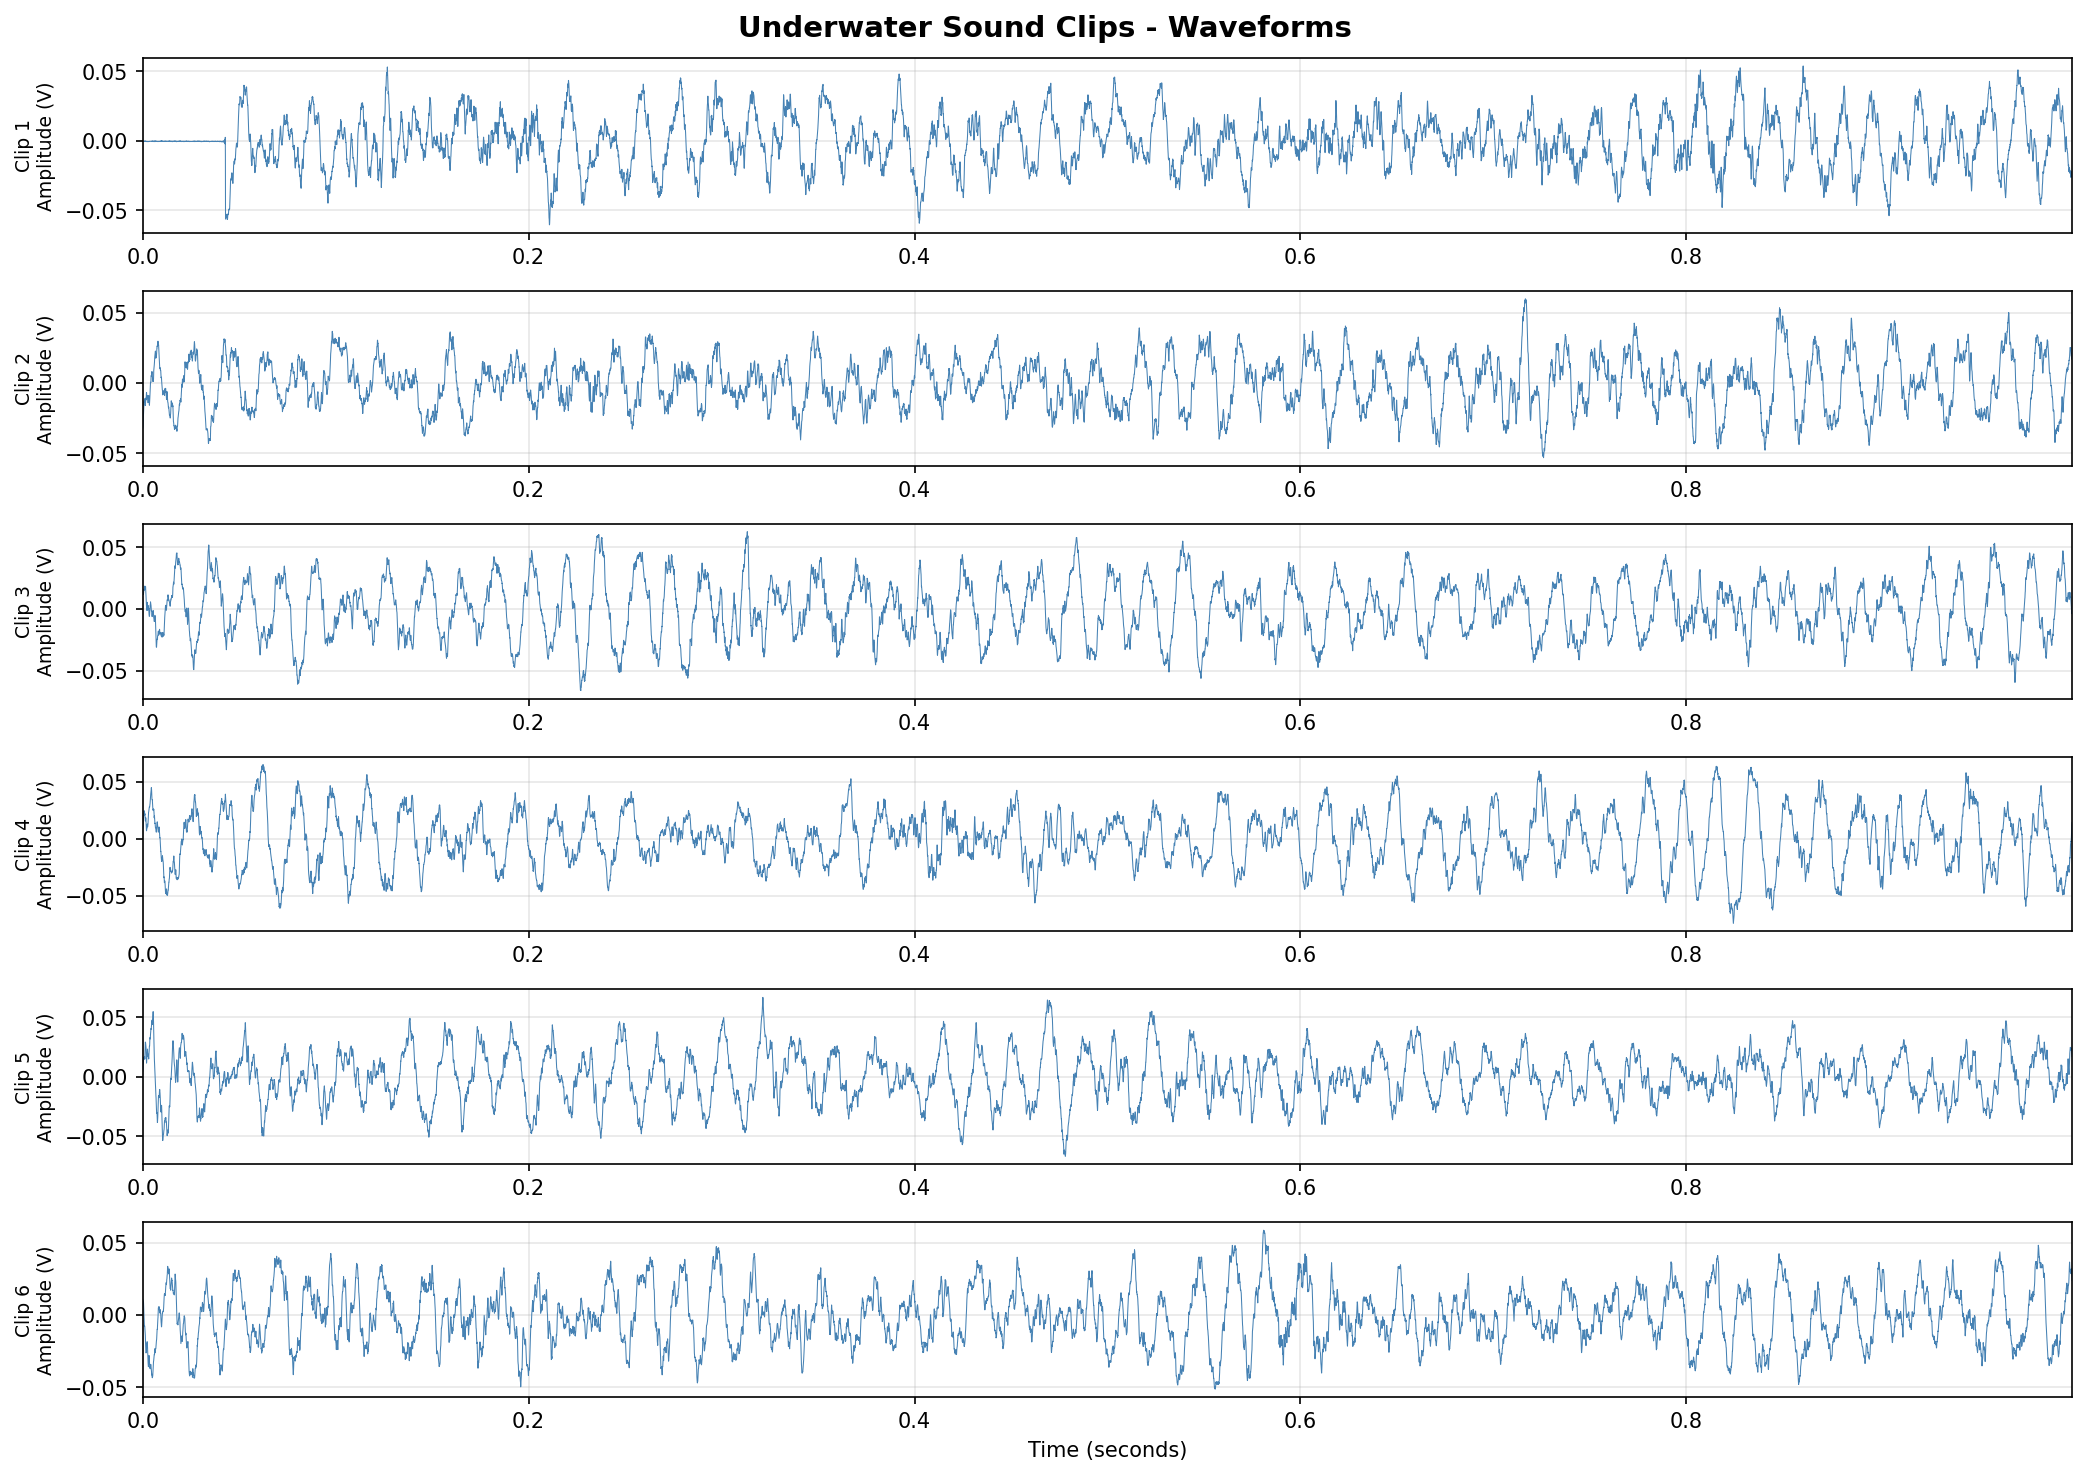
\includegraphics[width=0.95\textwidth]{01_waveforms.png}
    \caption{Time-domain waveforms of six underwater clips. X-axis: time (s), Y-axis: amplitude (V).}
\end{figure}

\begin{figure}[H]
    \centering
    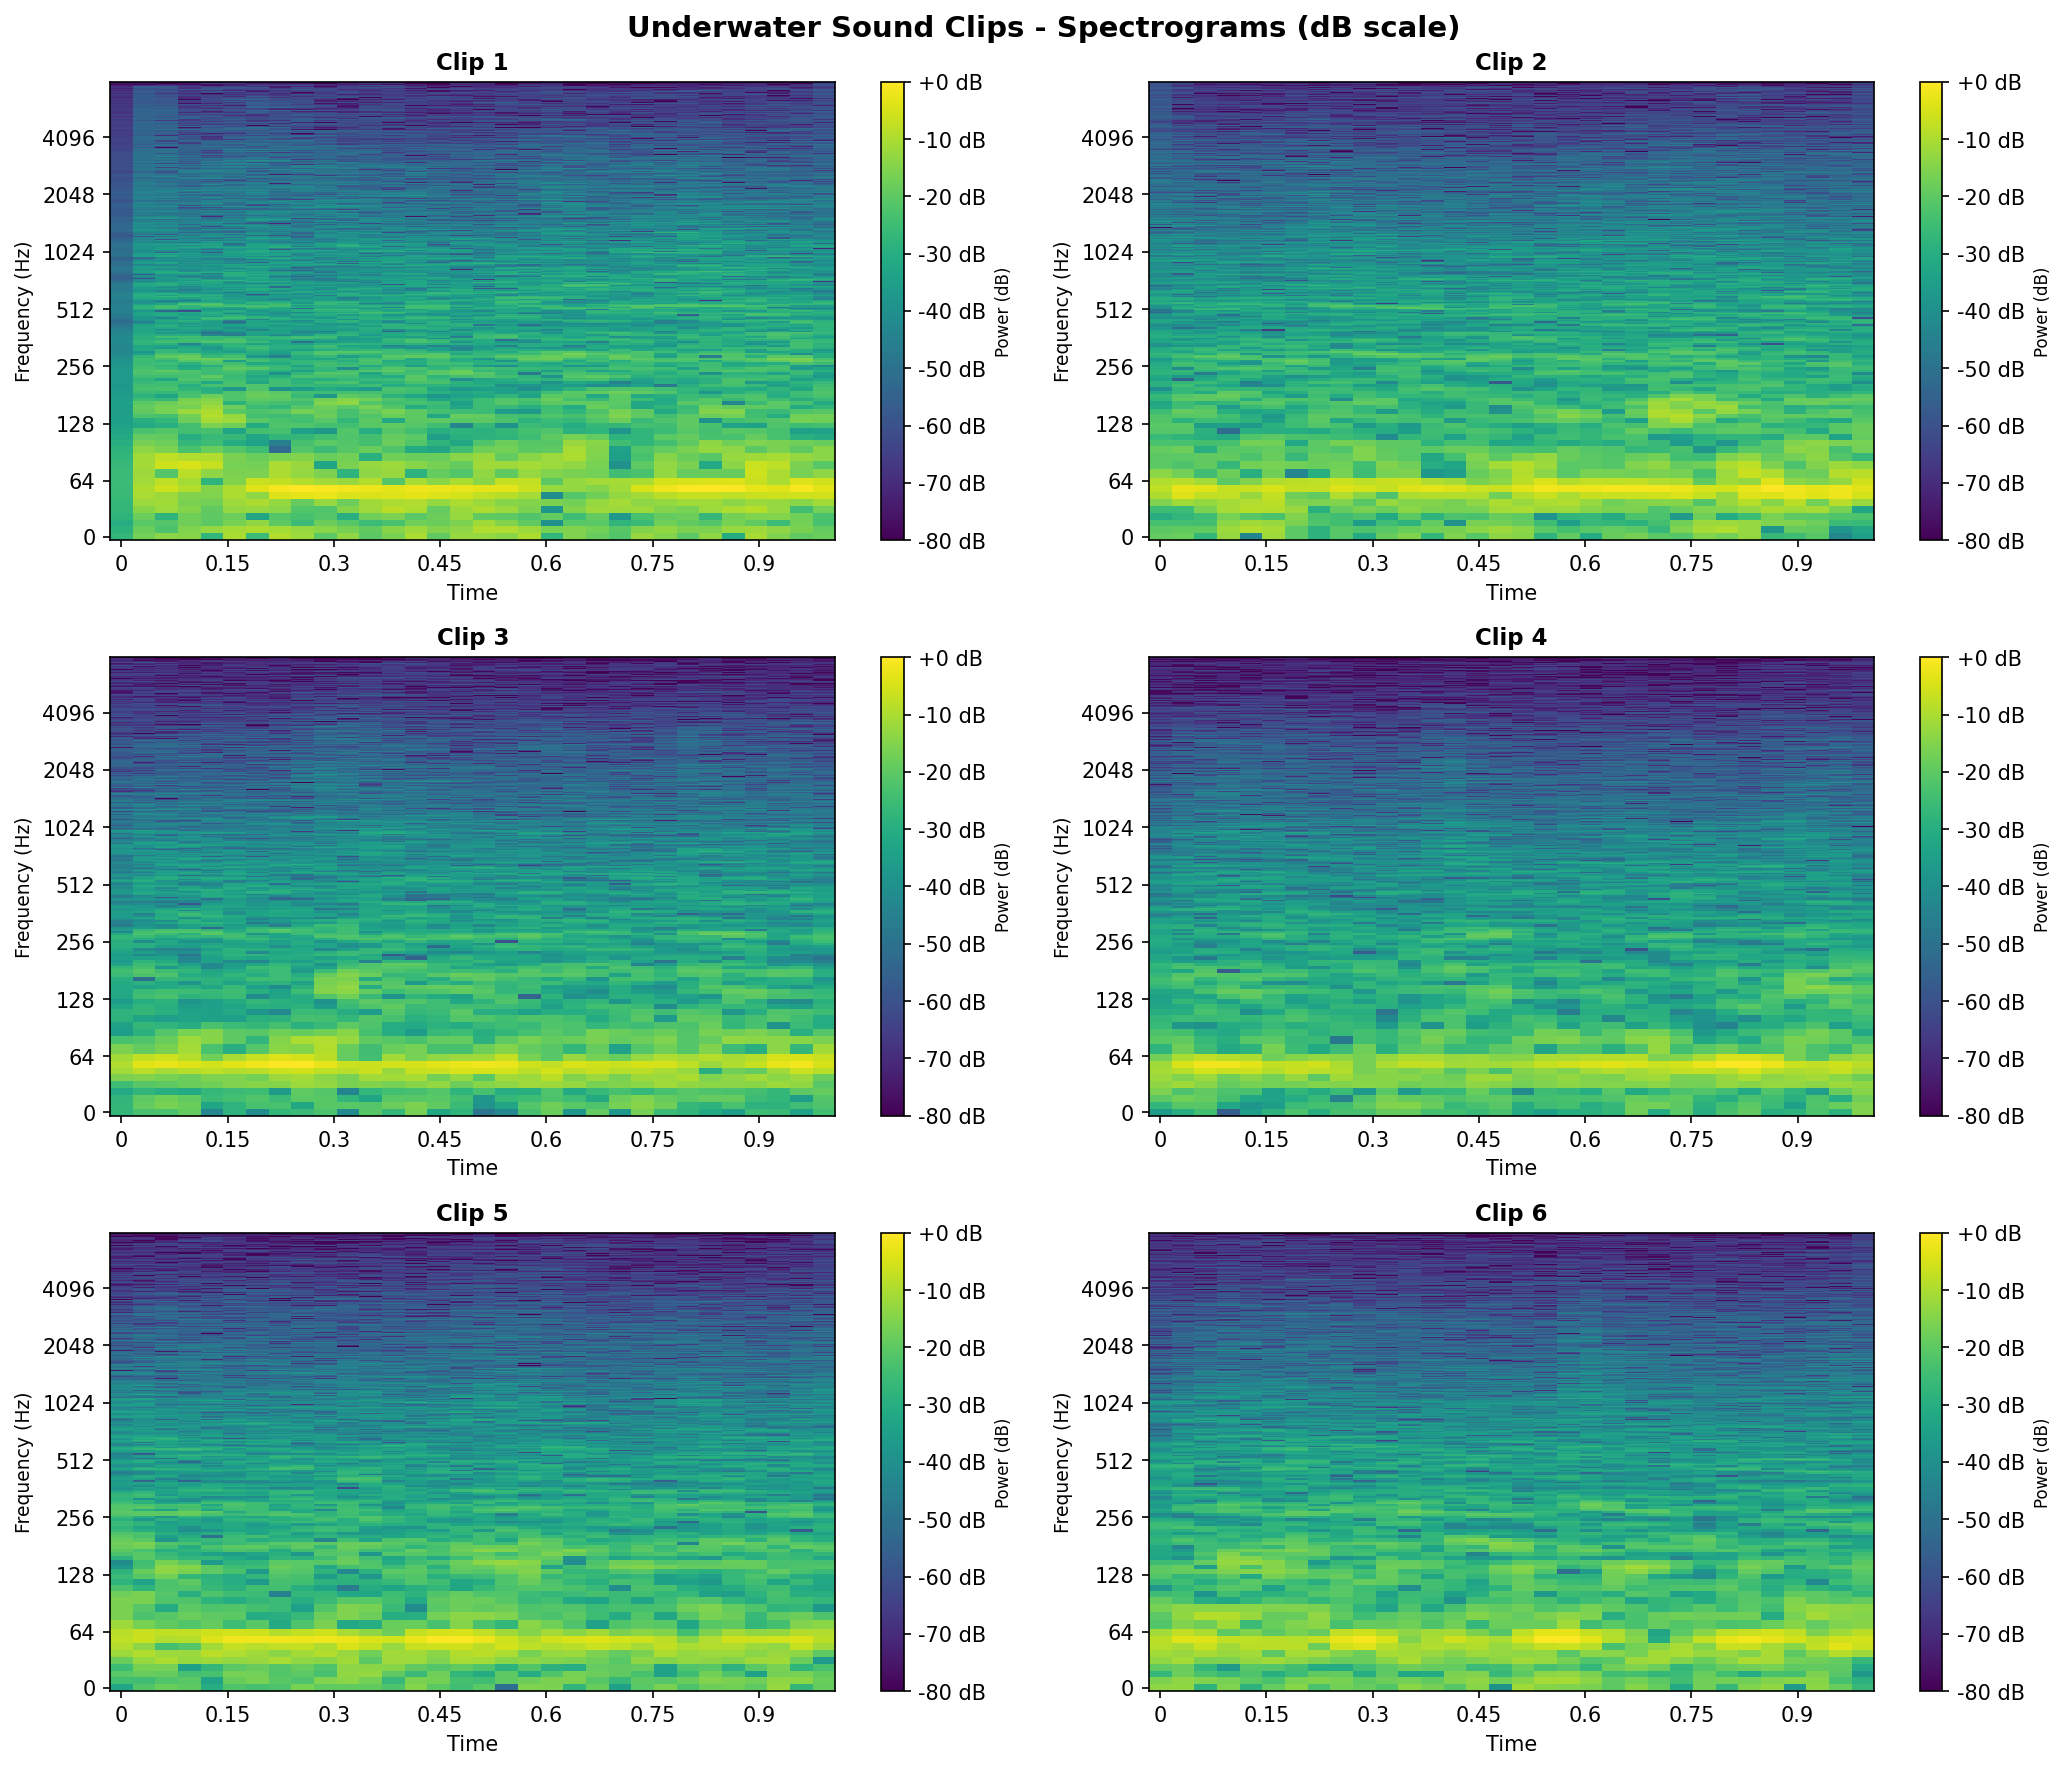
\includegraphics[width=0.95\textwidth]{02_spectrograms.png}
    \caption{Spectrograms of six clips. Axes: time (s) and frequency (Hz, log scale). Color: power (dB).}
\end{figure}

\begin{figure}[H]
    \centering
    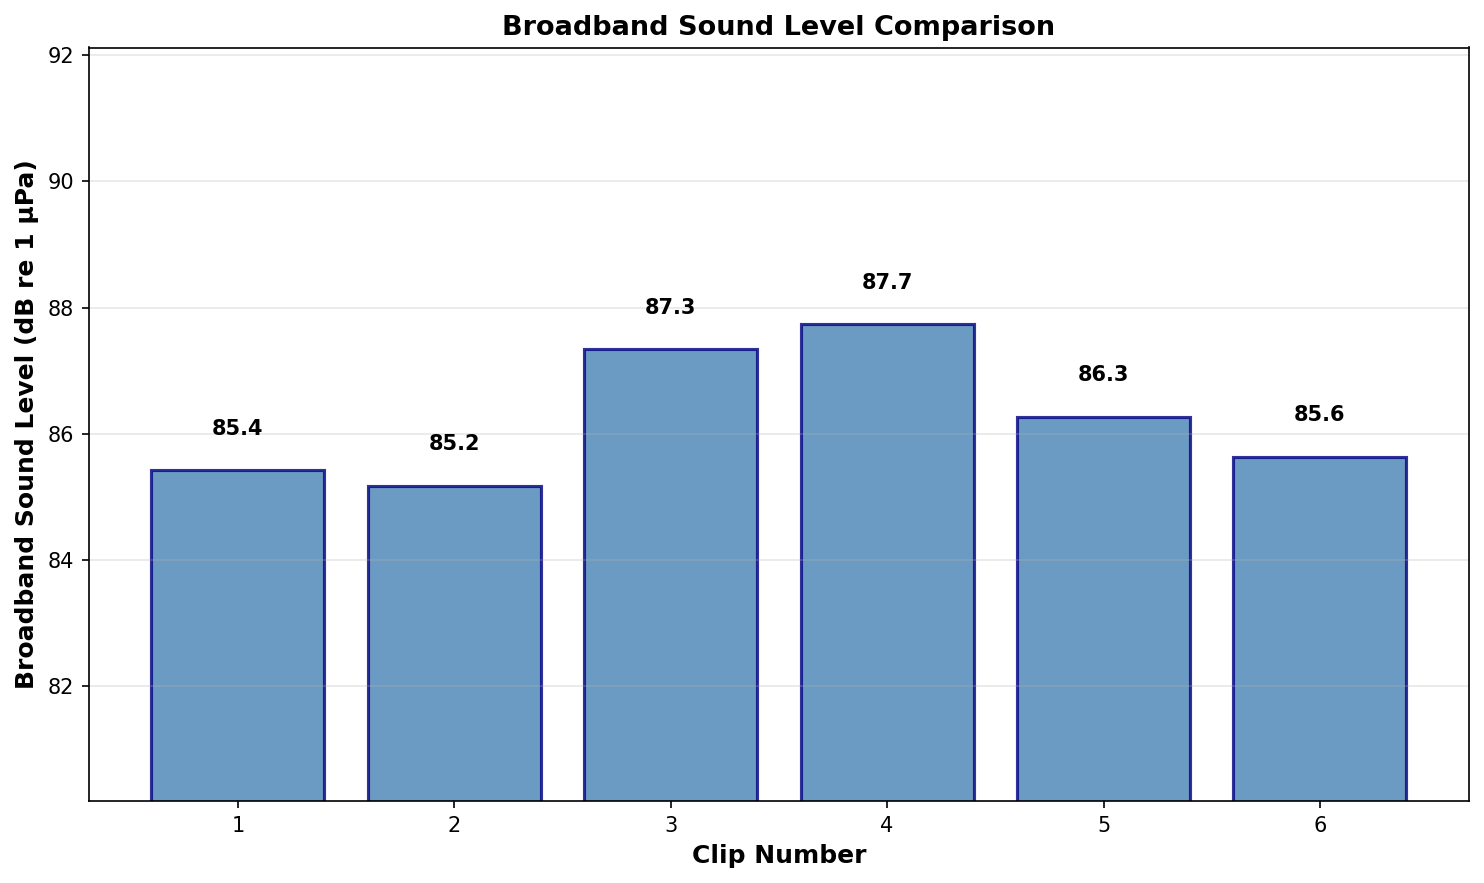
\includegraphics[width=0.8\textwidth]{03_broadband_levels.png}
    \caption{Broadband sound level comparison across clips. Unit: dB re \SI{1}{\micro\pascal}.}
\end{figure}

\begin{figure}[H]
    \centering
    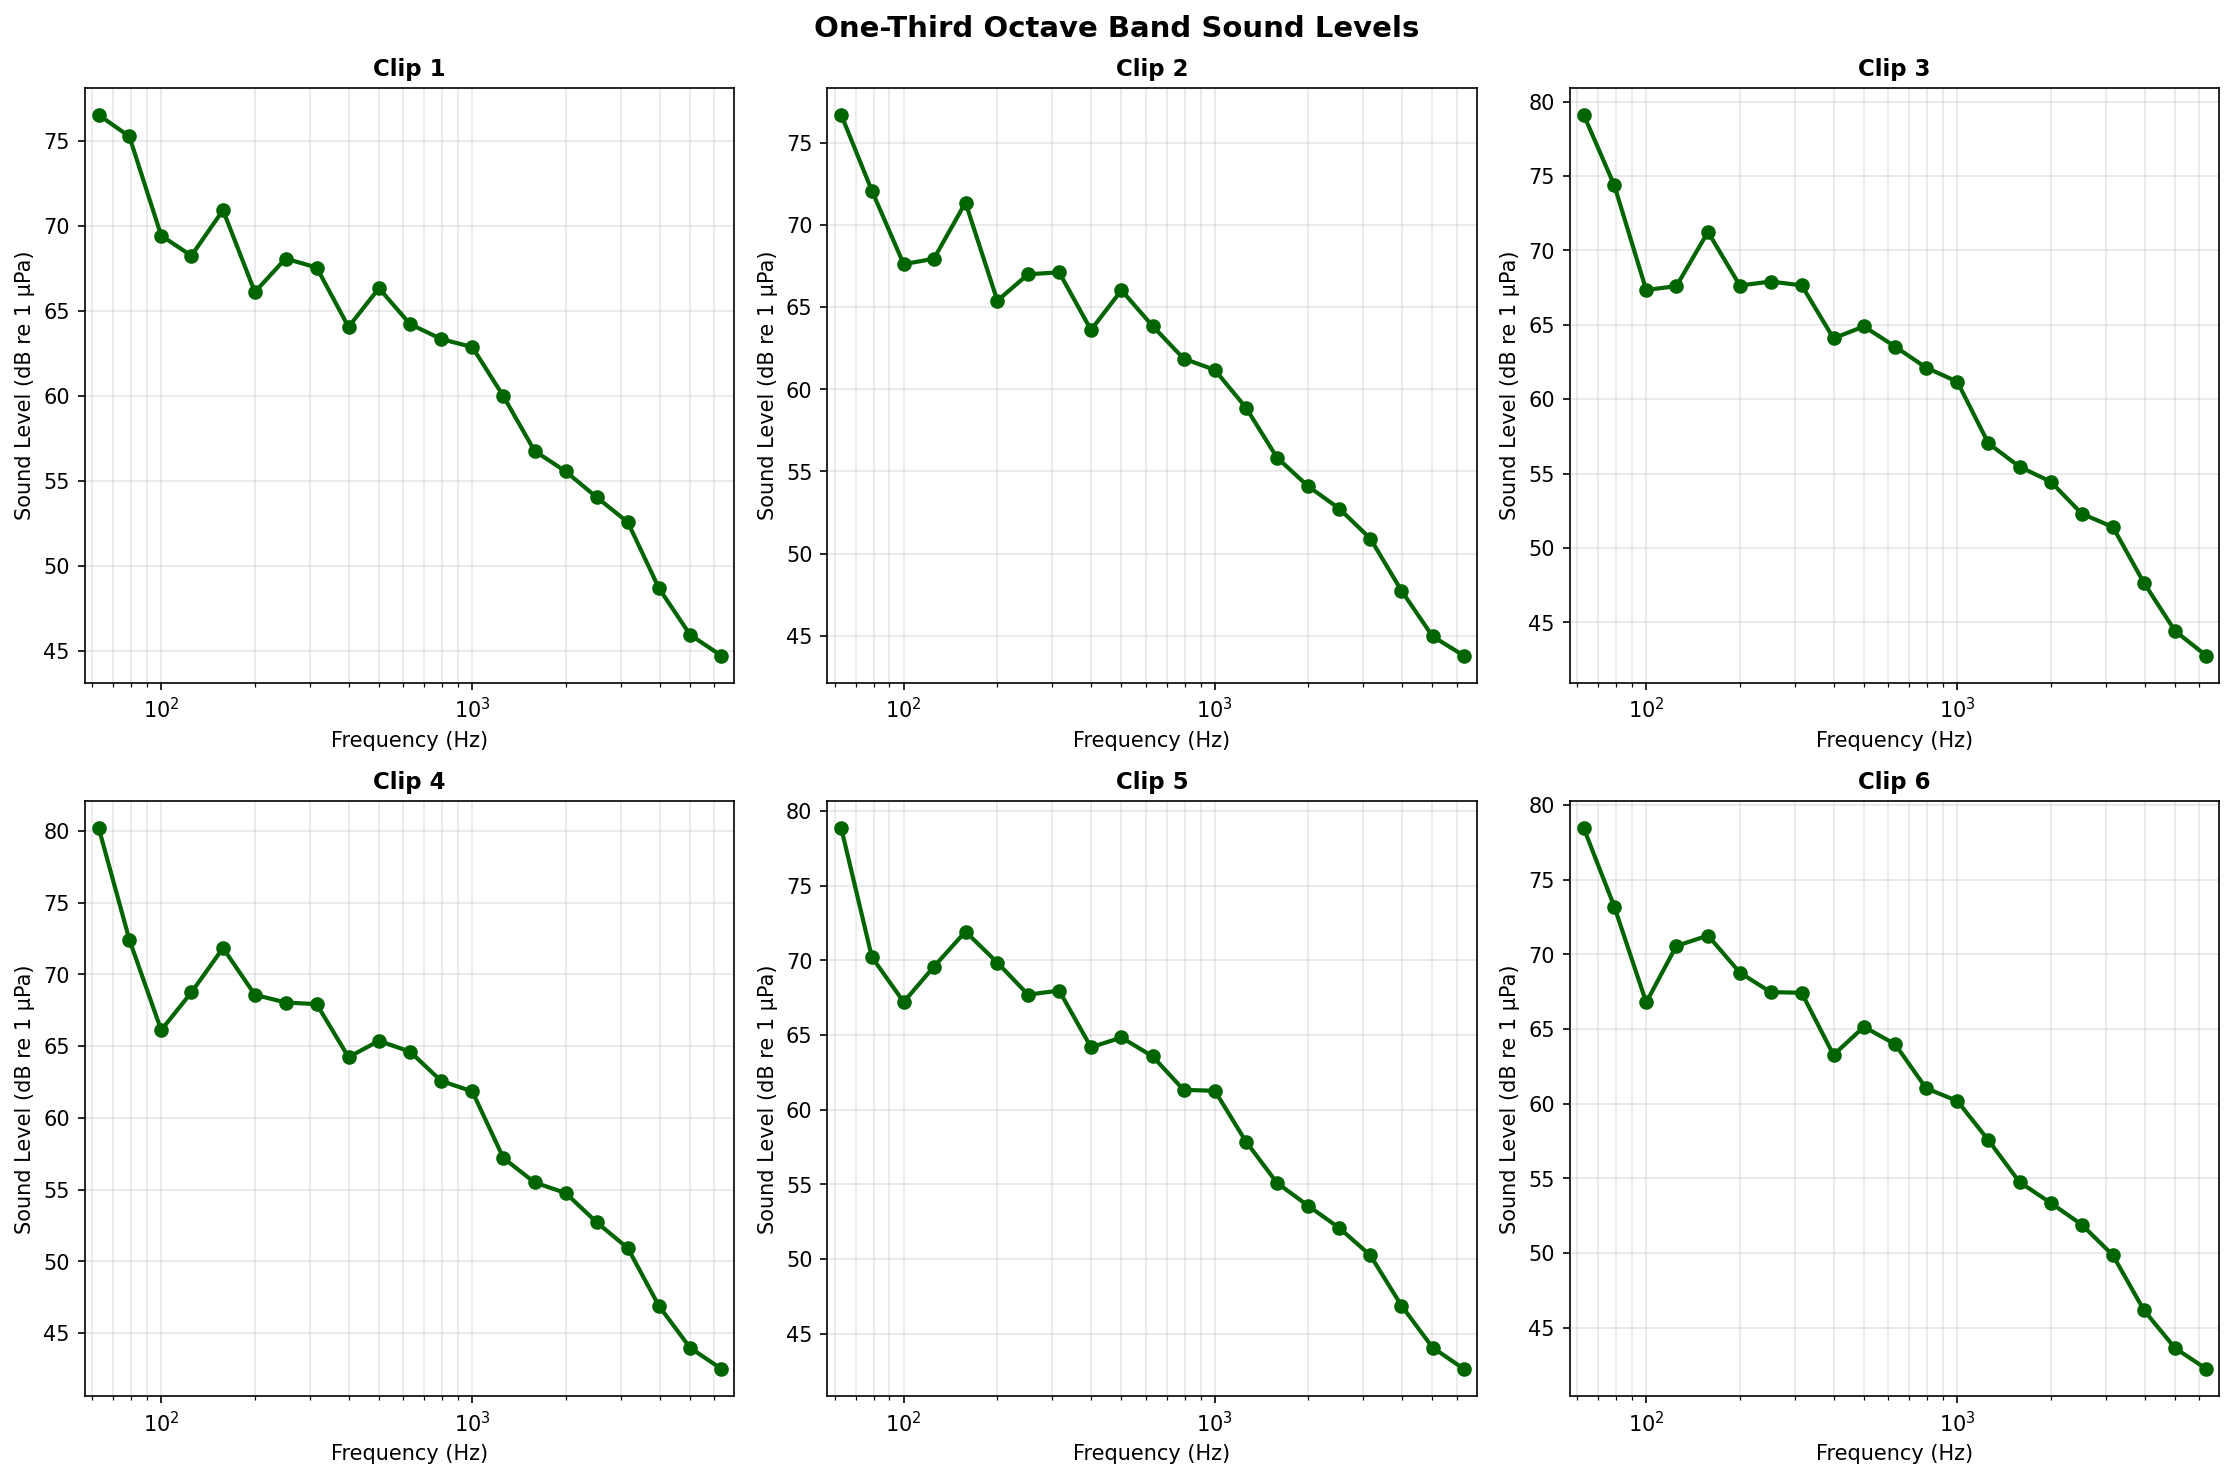
\includegraphics[width=0.95\textwidth]{04_octave_bands.png}
    \caption{One-third octave band levels for each clip. X-axis: frequency (Hz), Y-axis: level (dB re \SI{1}{\micro\pascal}).}
\end{figure}

\begin{figure}[H]
    \centering
    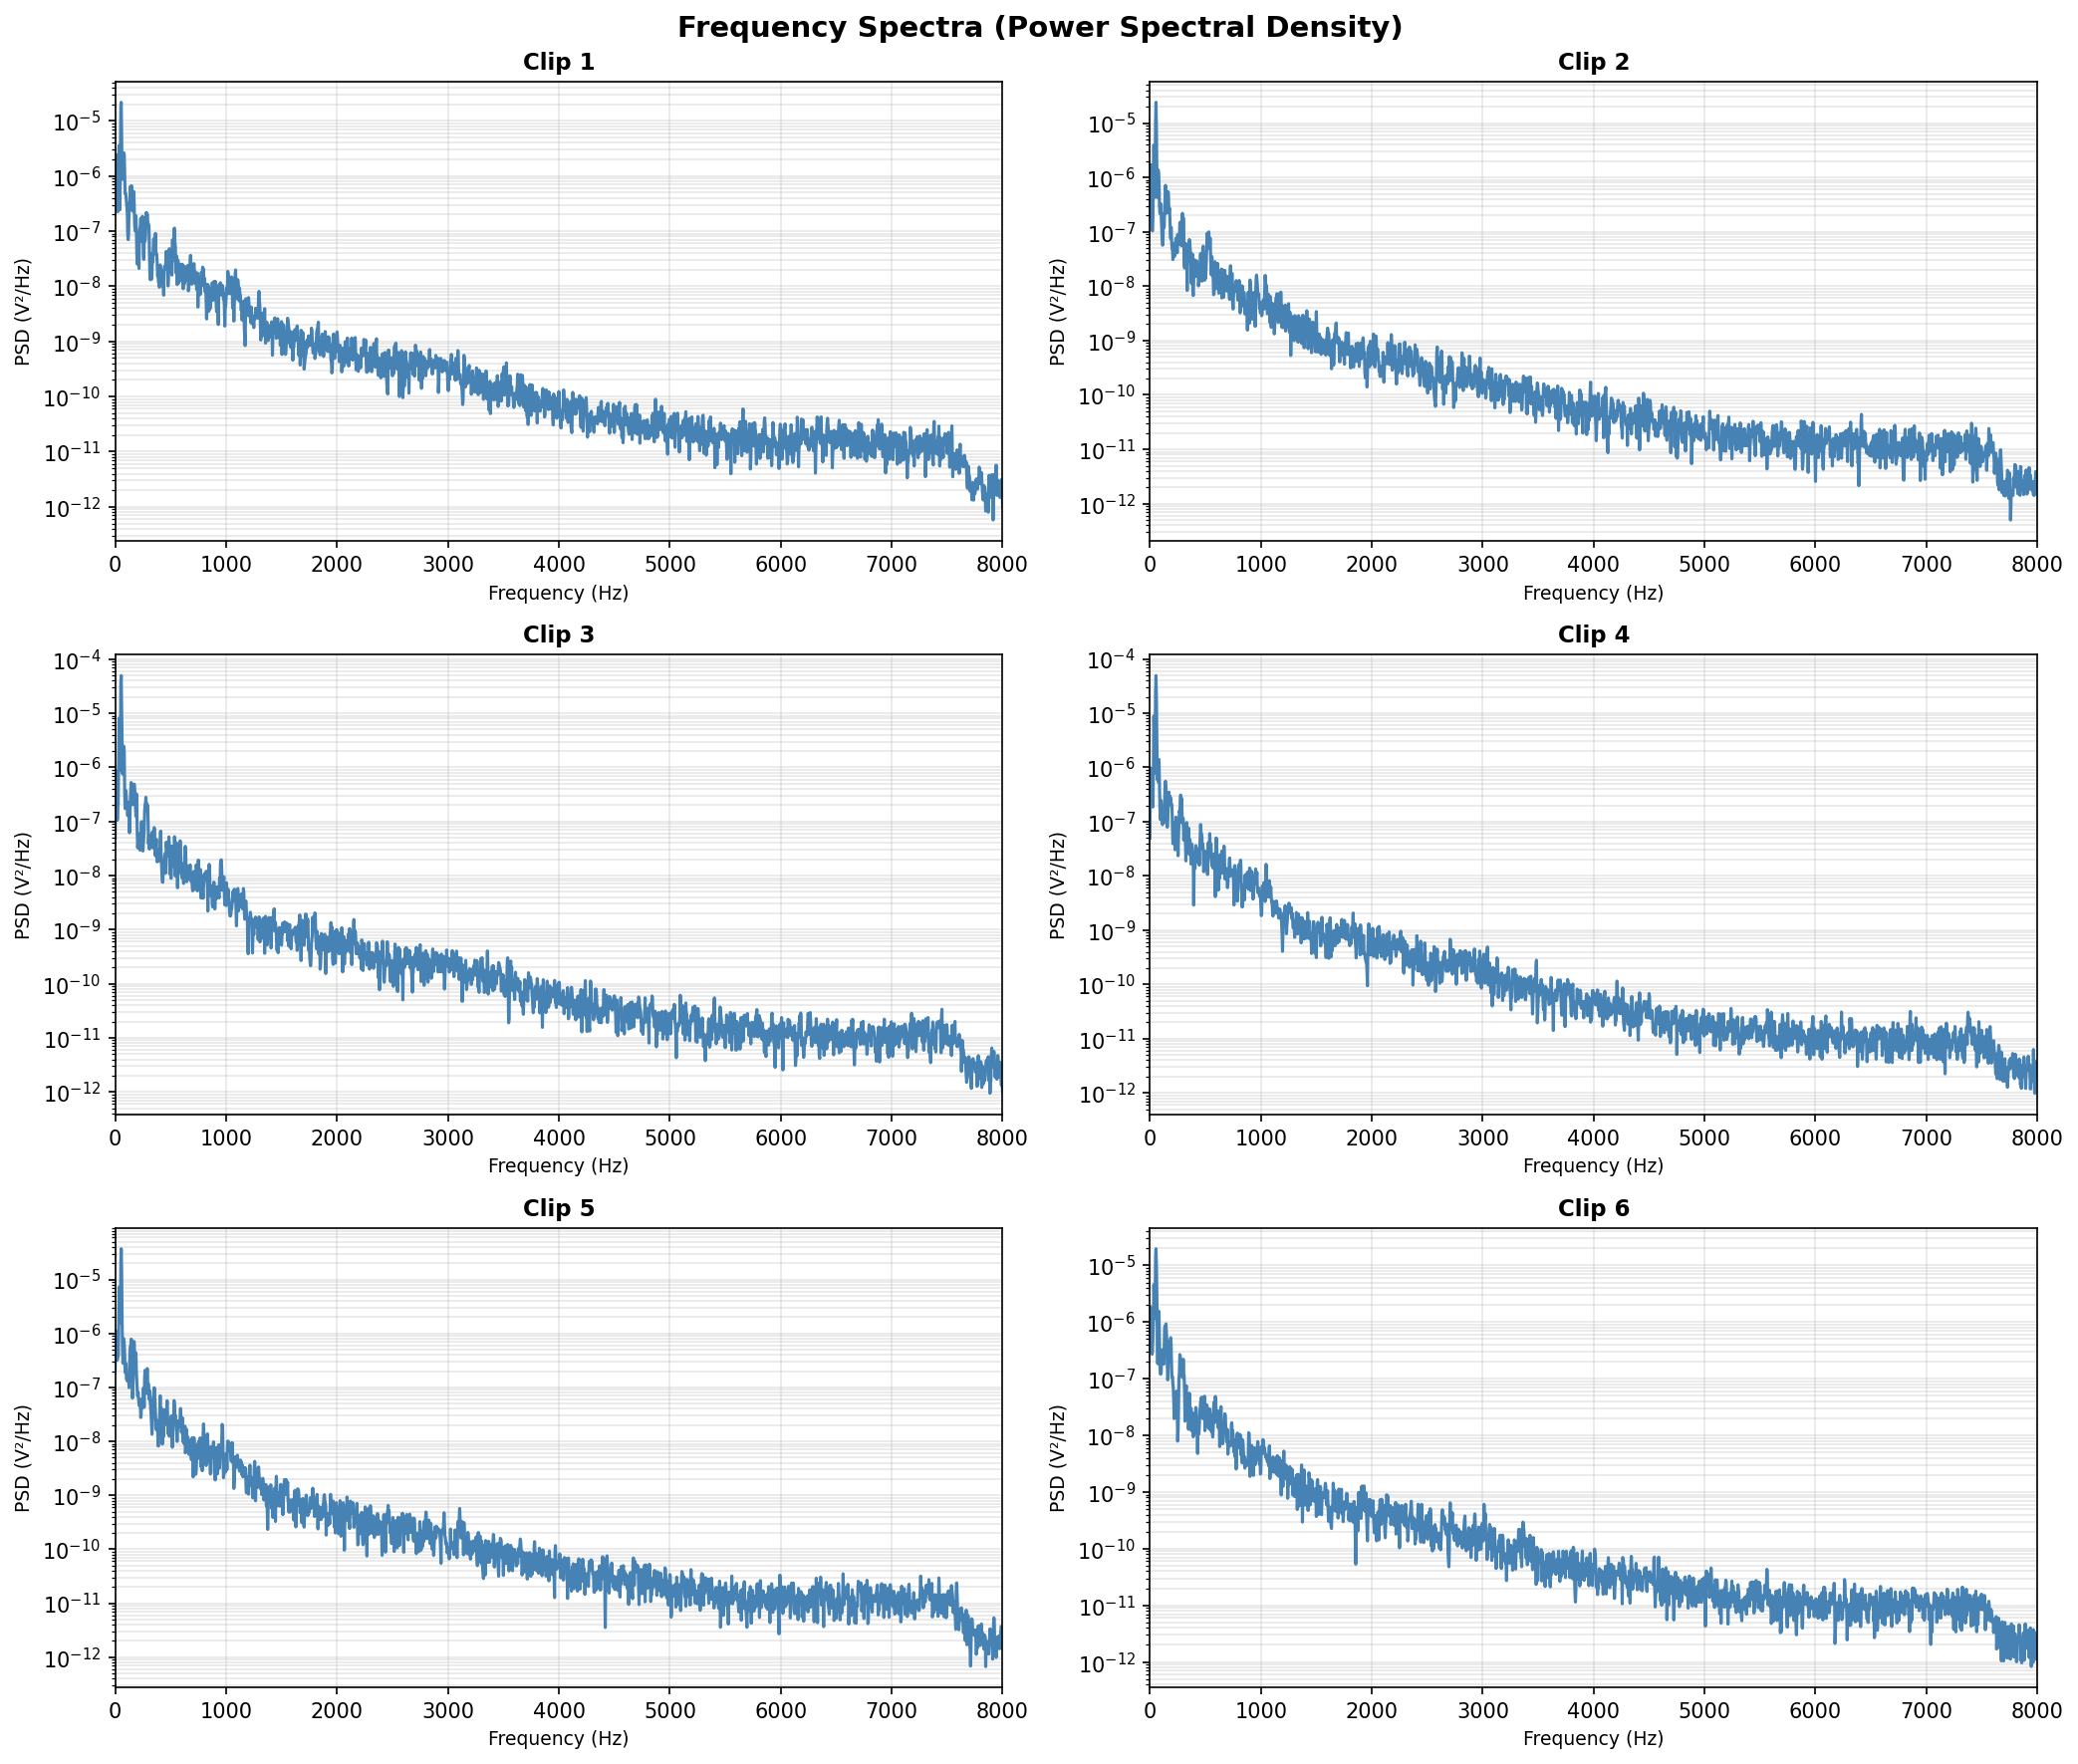
\includegraphics[width=0.95\textwidth]{05_frequency_spectra.png}
    \caption{Welch PSD for six clips. X-axis: frequency (Hz), Y-axis: PSD (V$^2$/Hz).}
\end{figure}

Putting all evidence together, the analyzed segment is most consistent with a quasi-continuous low-frequency source, likely mechanical in origin (for example vessel propulsion or nearby marine machinery). A biological source cannot be fully ruled out without contextual metadata, but the persistent narrow low-frequency dominance and stable level profile make a mechanical interpretation more plausible.

This report includes all required deliverables: unit-labeled plots, quantitative acoustic metrics, one-third octave analysis, and data-driven observations highlighting the most informative characteristics of the recording.

\end{document}
